\section{VNA Design Files}
\label{appen:vna_design_files}

All files used in the design of the VNA can be found at \url{https://github.com/joshajohnson/vna}. 
Some of the files, such as the schematic, images of the PCB, and functional block diagrams are included either in the body of this thesis, or in the following pages. 

Schematics for the test boards, ECal unit, along with the code written for the VNA is not included in the thesis, as there are numerous schematics and thousands of lines of code and as such appending them would not be reasonable. The below dot points link through to the GitHub repository where some of the key files can be found if desired. \\

\textbf{Hardware}
\begin{itemize}
	\item \href{https://github.com/joshajohnson/vna/tree/master/Hardware}{Hardware Folder}

\begin{itemize}
	\item \href{https://github.com/joshajohnson/vna/tree/master/Hardware/VNAv0}{KiCad Design Files for VNA}
	\item \href{https://github.com/joshajohnson/vna/tree/master/Hardware/VNAv0/gerbers}{VNA Gerbers}
	\item \href{https://github.com/joshajohnson/vna/tree/master/Hardware/VNAv0/renders_screenshots}{Renders and Screenshots of PCBA}
	\item \href{https://github.com/joshajohnson/vna/tree/master/Hardware/Test\%20Boards}{Functional Block Evaluation Boards}
	\item \href{https://github.com/joshajohnson/vna/tree/master/Hardware/Ecal}{ECal Hardware Design}\\
\end{itemize}
\end{itemize}

\textbf{Firmware}
\begin{itemize}
	\item \href{https://github.com/joshajohnson/vna/tree/master/Firmware/VNA}{Firmware Files for VNA} 
	\begin{itemize}
		\item \href{https://github.com/joshajohnson/vna/blob/master/Firmware/VNA/Src/max2871.c}{MAX2871 Programming}
		\item
		\href{https://github.com/joshajohnson/vna/blob/master/Firmware/VNA/Src/max2871_registers.c}{MAX2871 Register Configuration}
		\item
		\href{https://github.com/joshajohnson/vna/blob/master/Firmware/VNA/Src/txChain.c}{Transmit Chain Control}
		\item
		\href{https://github.com/joshajohnson/vna/blob/master/Firmware/VNA/Src/receiver.c}{AD8302 Measurement and Initial Phase Correction}
		\item
		\href{https://github.com/joshajohnson/vna/blob/master/Firmware/VNA/Src/commandParser.c}{Command Parsing and VNA Control}
	\end{itemize}
	\item \href{https://github.com/joshajohnson/vna/tree/master/Firmware/DevBoards}{Firmware Targeting Development Boards}\\
\end{itemize}


\textbf{Software}
\begin{itemize}
	\item \href{https://github.com/joshajohnson/vna/tree/master/Software/vna}{Software Folder}
	\begin{itemize}
		\item \href{https://github.com/joshajohnson/vna/blob/master/Software/vna/vna.py}{VNA Control Software}
		\item \href{https://github.com/joshajohnson/vna/blob/master/Software/vna/phase_correction.ipynb}{Phase Correction Jupyter Notebook}
		\item \href{https://github.com/joshajohnson/vna/blob/master/Software/justTesting/ad8302Cal.m}{MATLAB Phase Compensation Script}
		\item \href{https://github.com/joshajohnson/vna/blob/master/Software/vna/calibration.ipynb}{Calibration Jupyter Notebook}
		\item \href{https://github.com/joshajohnson/vna/blob/master/Firmware/DevBoards/freqGen.py}{Python Implementation of PLL Configuration}
	\end{itemize}
\end{itemize}



\begin{landscape}
	
	\begin{figure}
		\centering
		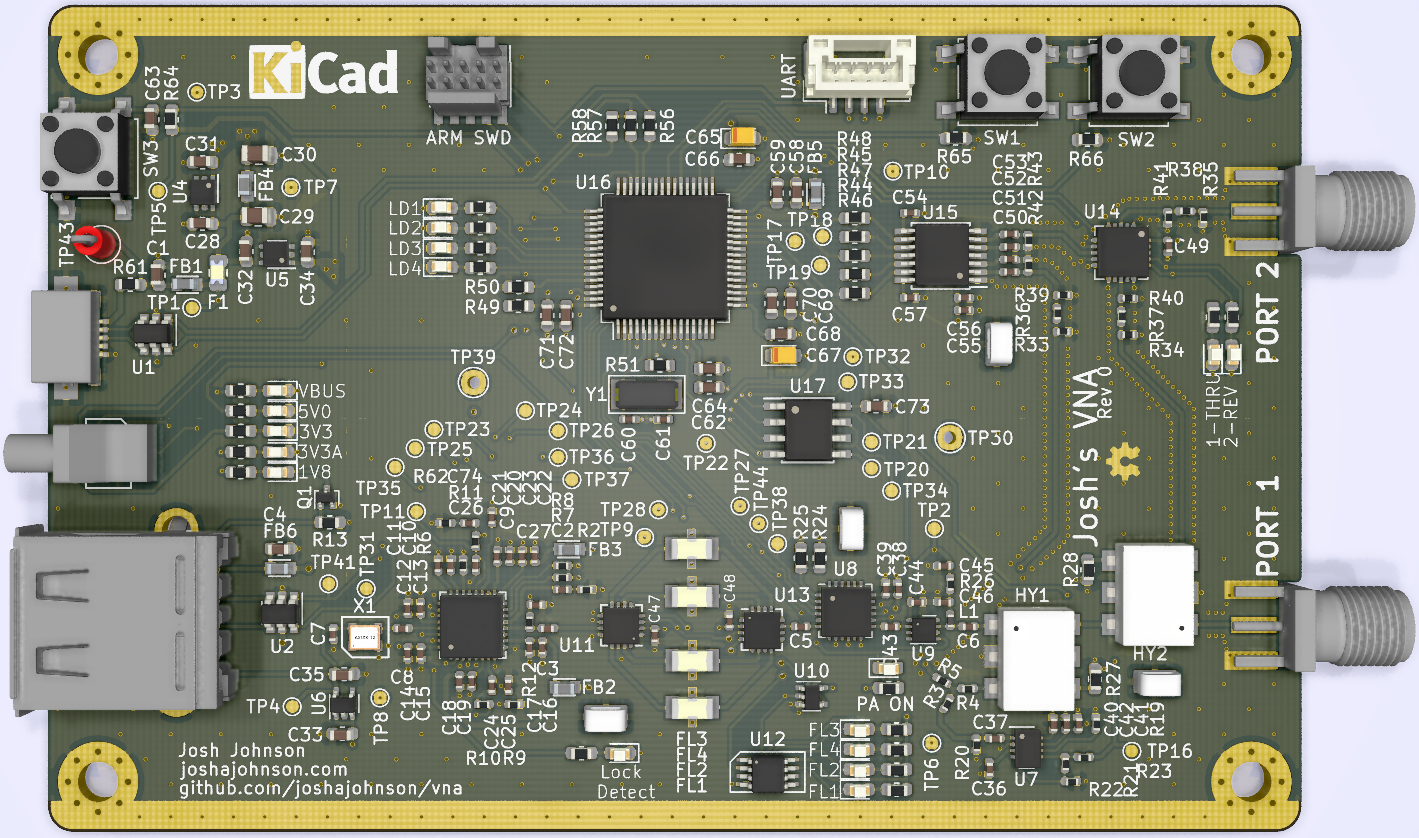
\includegraphics[width=\linewidth]{thirdDayRender.png}
		\caption{3D render of the PCB}
		\label{fig:pcb_render}
	\end{figure}

	\begin{figure}
		\centering
		\includegraphics[width=\linewidth, page = 1]{vna.pdf}
		\caption{VNA Schematic - Overview}
		\label{fig:vna_schematic_overview}
	\end{figure}

	\begin{figure}
		\centering
		\includegraphics[width=\linewidth, page = 2]{vna.pdf}
		\caption{VNA Schematic - LO Generation}
		\label{fig:vna_schematic_lo}
	\end{figure}
	
	\begin{figure}
		\centering
		\includegraphics[width=\linewidth, page = 6]{vna.pdf}
		\caption{VNA Schematic - Filter Bank}
		\label{fig:vna_schematic_filter}
	\end{figure}
	
	\begin{figure}
		\centering
		\includegraphics[width=\linewidth, page = 4]{vna.pdf}
		\caption{VNA Schematic - Source Levelling}
		\label{fig:vna_schematic_source_levelling}
	\end{figure}
	
	\begin{figure}
		\centering
		\includegraphics[width=\linewidth, page = 5]{vna.pdf}
		\caption{VNA Schematic - Coupling}
		\label{fig:vna_schematic_coupling}
	\end{figure}
	
	\begin{figure}
		\centering
		\includegraphics[width=\linewidth, page = 7]{vna.pdf}
		\caption{VNA Schematic - Gain and Phase Detection}
		\label{fig:vna_schematic_ad8302}
	\end{figure}
	
	\begin{figure}
		\centering
		\includegraphics[width=\linewidth, page = 8]{vna.pdf}
		\caption{VNA Schematic - Microcontroller}
		\label{fig:vna_schematic_micro}
	\end{figure}
	
	\begin{figure}
		\centering
		\includegraphics[width=\linewidth, page = 3]{vna.pdf}
		\caption{VNA Schematic - Power}
		\label{fig:vna_schematic_power}
	\end{figure}
\end{landscape}

\section{Board Images}
Below are a number of images which were taken during development and may of be interest, however are not directly relevant to function of the device. 

\begin{figure}[H]
	\centering
	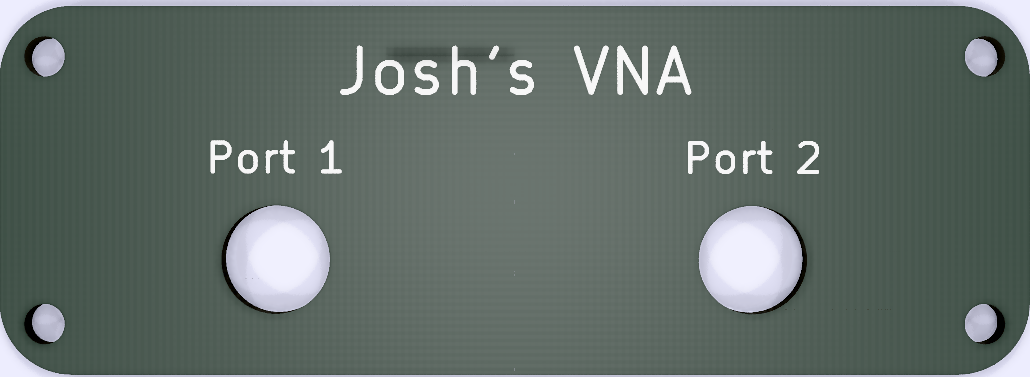
\includegraphics[width=0.8\linewidth]{frontPanel.png}
	\caption{Render of the VNA Front Panel}
	\label{fig:pcb_front_render}
\end{figure}

\begin{figure}[H]
	\centering
	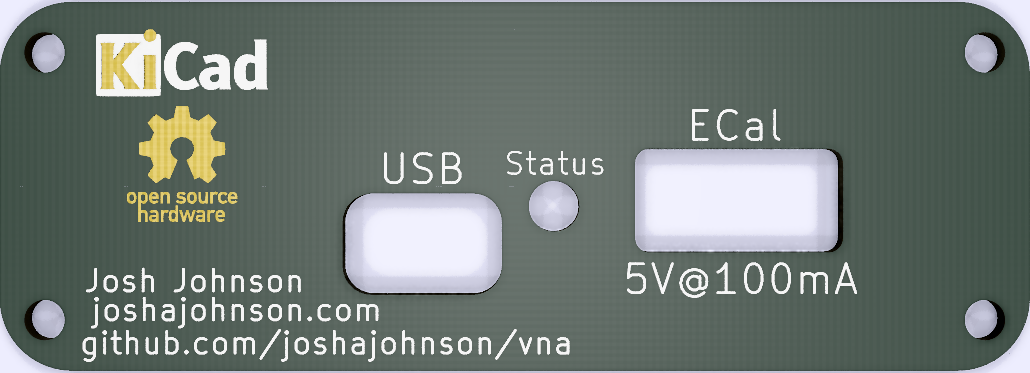
\includegraphics[width=0.8\linewidth]{rearPanel.png}
	\caption{Render of the VNA Rear Panel}
	\label{fig:pcb_rear_render}
\end{figure}

\begin{figure}[H]
	\centering
	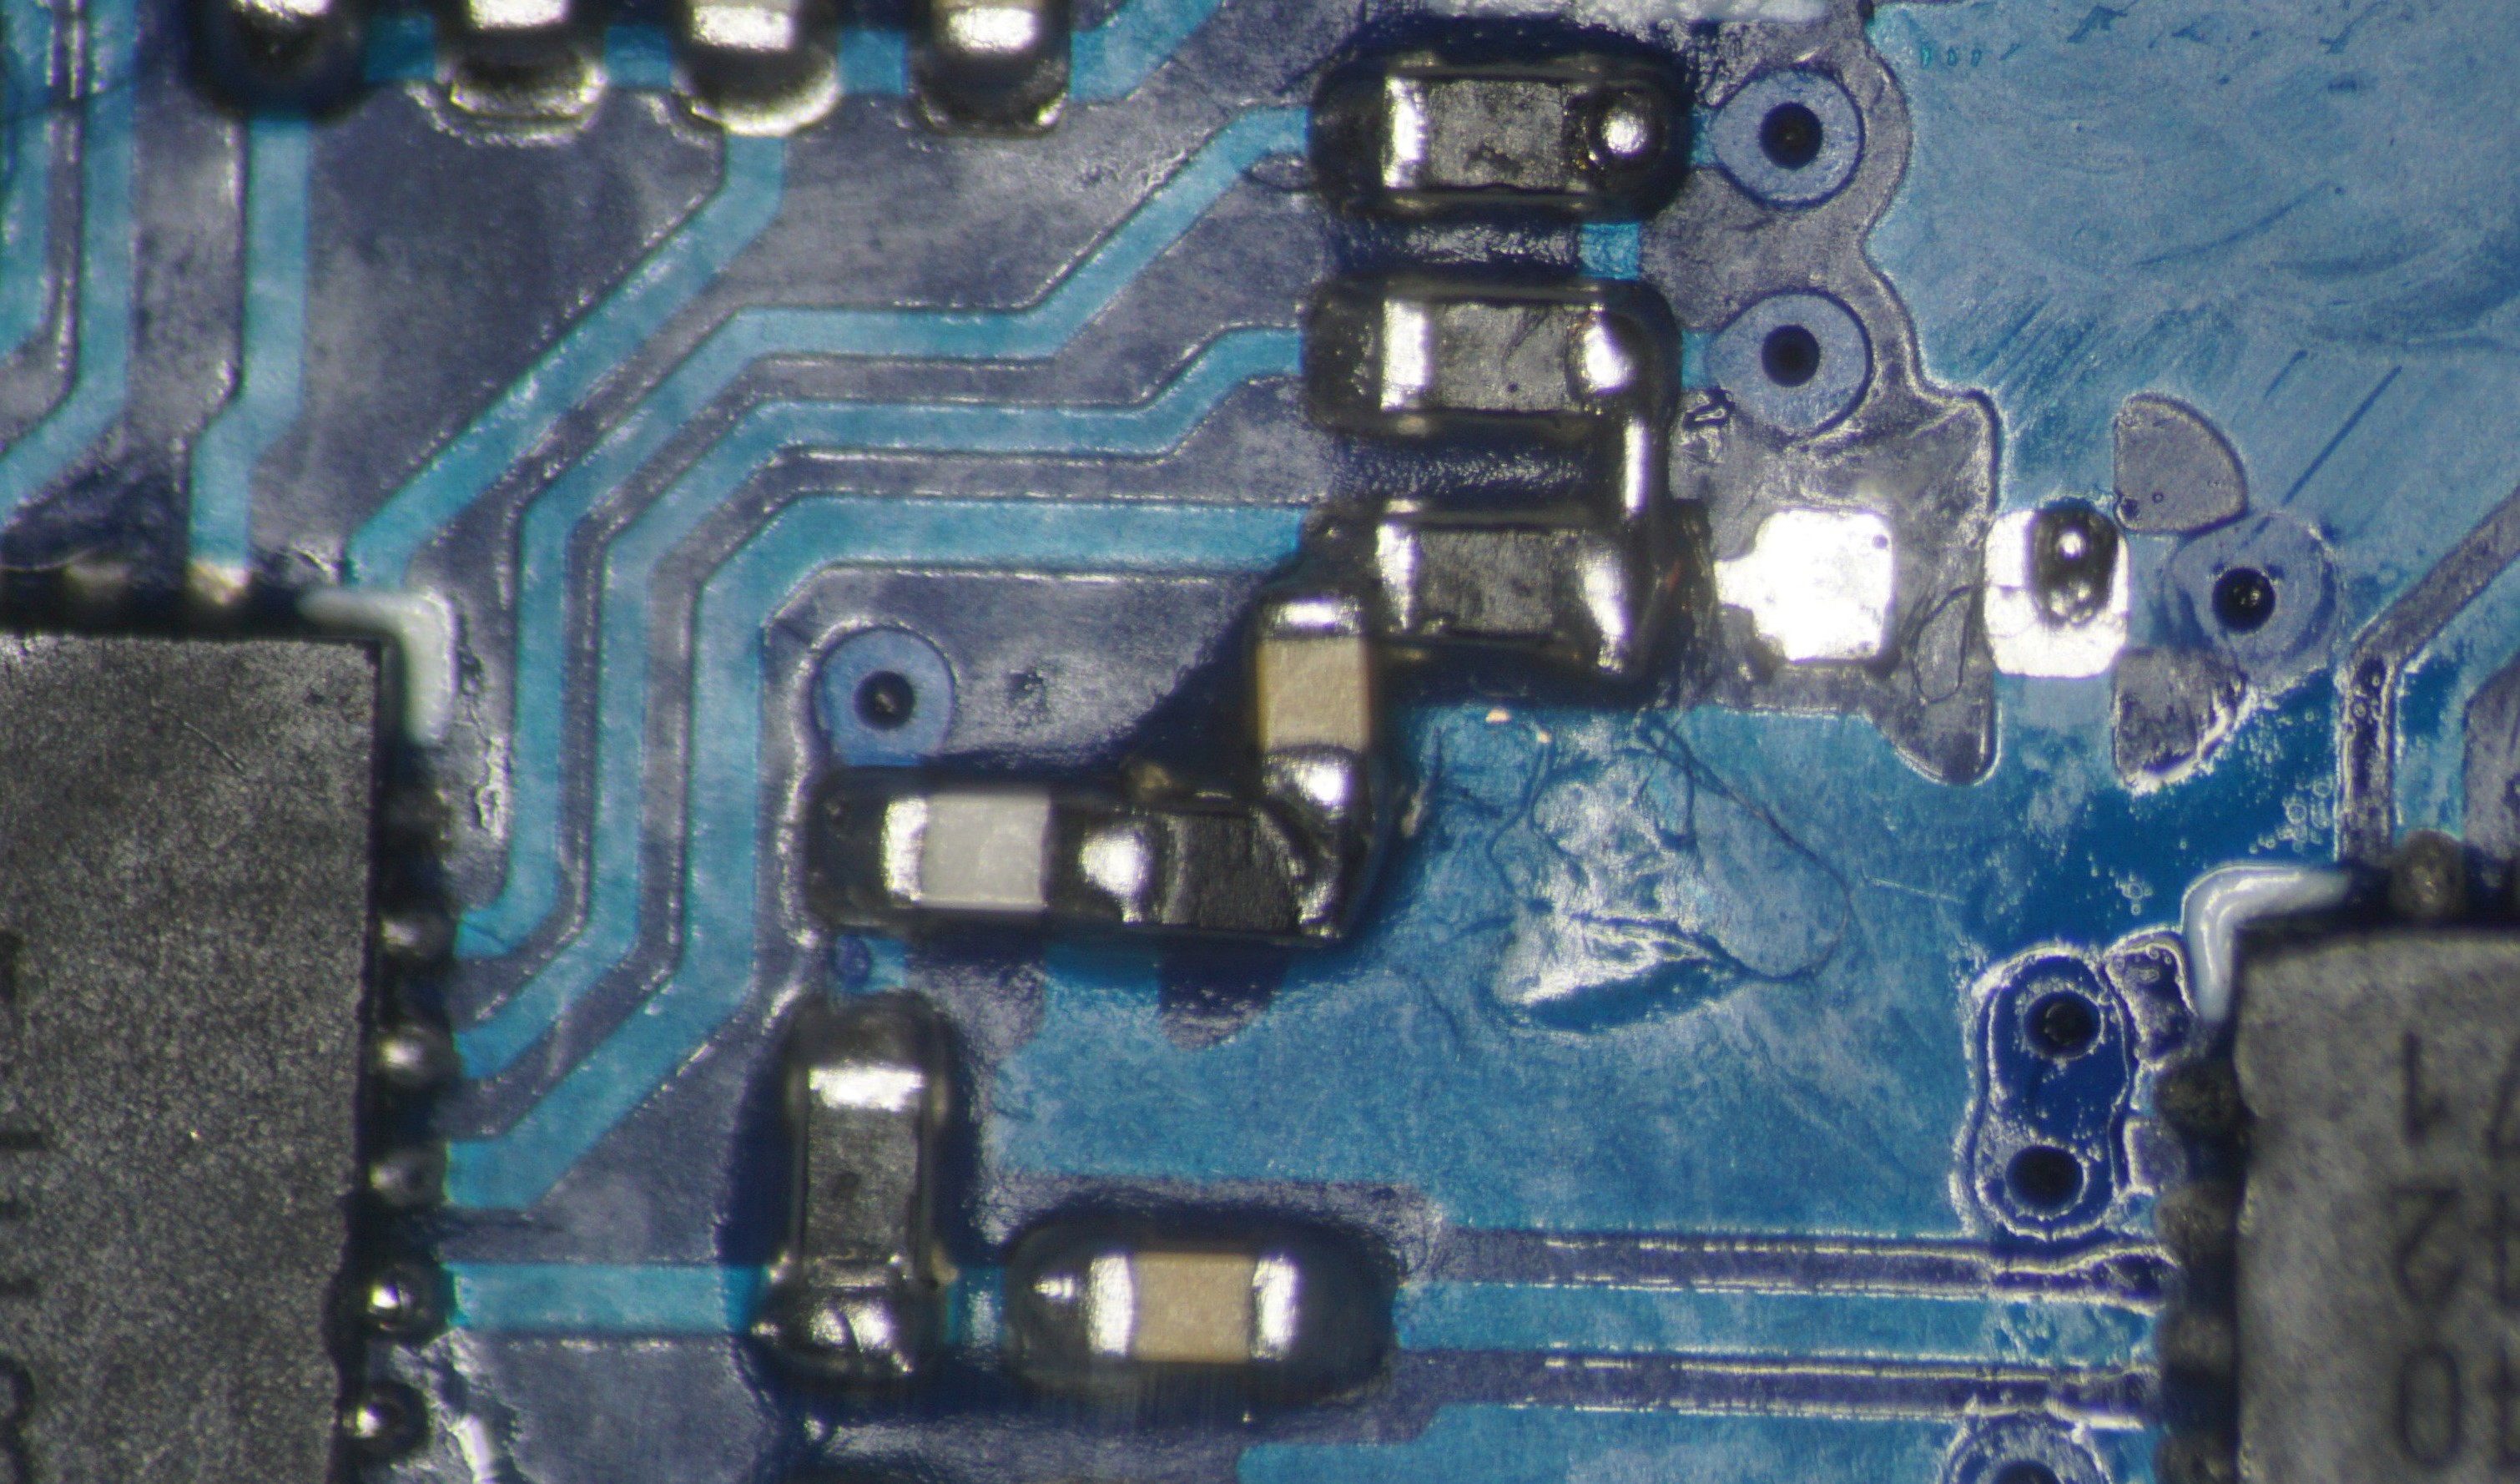
\includegraphics[width=0.65\linewidth]{max_rework.jpg}
	\caption{Rework of the MAX2871 RF- output}
	\label{fig:max_rework}
\end{figure}


\begin{figure}[H]
	\centering
	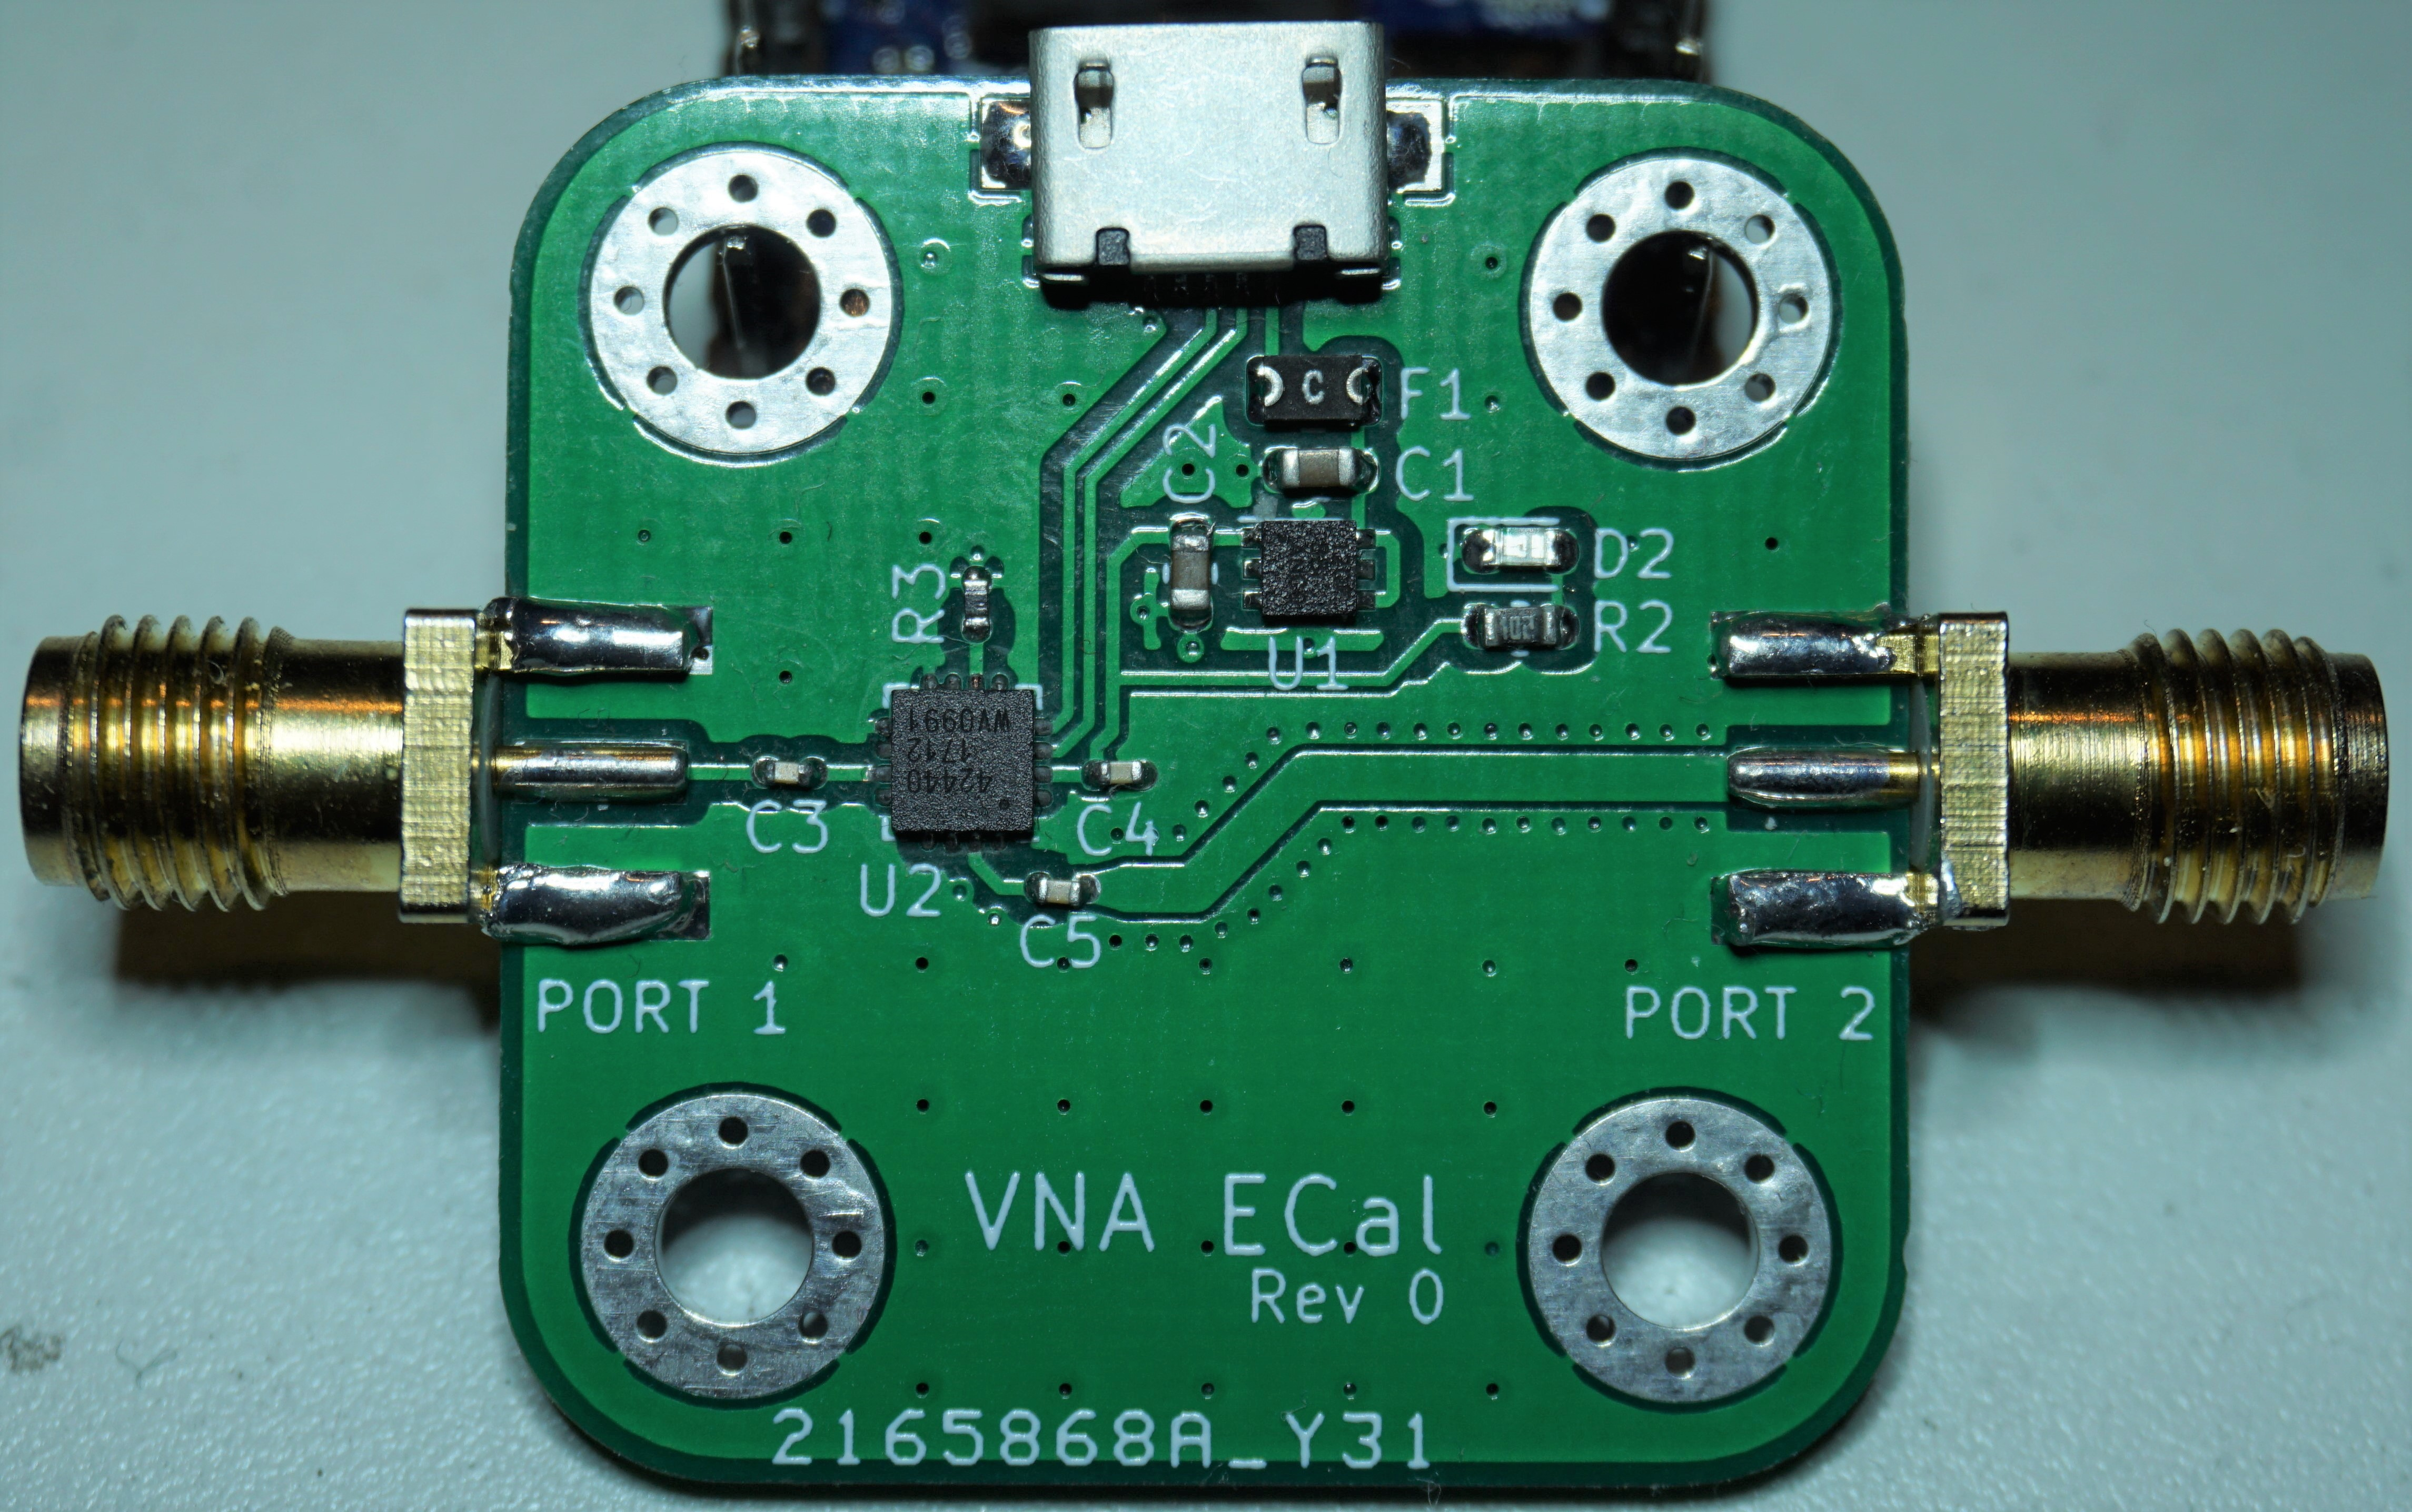
\includegraphics[width=0.65\linewidth]{ecal_board.jpg}
	\caption{Image of the ECal Unit}
	\label{fig:ecal_photo}
\end{figure}